\documentclass{../../../oss-apphys-exam}
\usepackage{bm}

%\raggedcolumns

\runningheader{
  \fontfamily{phv}\small
  \textcolor{gray}{AP PHYSICS C: ELECTRICITY AND MAGNETISM $\blacksquare$}
  \textbf{FREE-RESPONSE QUESTIONS}}{}{}

\begin{document}
%\genheader

\gentitle{15}{HALL EFFECT AND MAXWELL'S EQUATIONS}

% TAKEN FROM THE 2009 AP PHYSICS C FREE-RESPONSE QUESTION E&M 2. THIS IS A
% HALL-EFFECT QUESTION
\cpic{.45}{hall2}
\begin{questions}
  \question A \SI{9.0}{\volt} battery is connected to a rectangular bar of
  length \SI{0.080}{\metre}, uniform cross-sectional area
  \SI{5.0e-6}{\metre\squared}, and resistivity \SI{4.5e-4}{\ohm\metre}, as
  shown above. Electrons are the sole charge carriers in the bar. The wires
  have negligible resistance. The switch in the circuit is closed at time $t=0$.

  \begin{parts}
    \part\textbf{Calculate} the power delivered to the circuit by the battery.
    \vspace{\stretch1}
    
    \part On the diagram below, \textbf{indicate} the direction of the electric
    field in the bar.
    \begin{center}
      \vspace{.2in}
      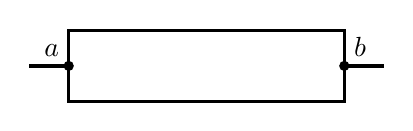
\begin{tikzpicture}[scale=.5]
        \draw[very thick](.5,.6) rectangle(7.5,2.4);
        \draw[very thick](-.5,1.5)--(.5,1.5);
        \draw[very thick](7.5,1.5)--(8.5,1.5);
        \fill(.5,1.5) circle(.13) node[above left] {$a$};
        \fill(7.5,1.5) circle(.13) node[above right]{$b$};
      \end{tikzpicture}\\
      Side View
      \vspace{.2in}
    \end{center}
    \textbf{Explain} your answer.
    \vspace{\stretch1}
    
    \part\textbf{Calculate} the strength of the electric field in the bar.
    \vspace{\stretch1}
    \newpage
    
    \uplevel{
      A uniform magnetic field of magnitude \SI{.25}{\tesla} perpendicular to
      the bar is added to the region around the bar, as shown below.
      \cpic{.8}{hall1}
    }

    \part\textbf{Calculate} the magnetic force on the bar.
    \vspace{\stretch1}
    
    \part The electrons moving through the bar are initially deflected by the
    external magnetic field. On the diagram below, indicate the direction of
    the additional electric field that is created in the bar by the deflected
    electrons.
    \begin{center}
      \vspace{.1in}
      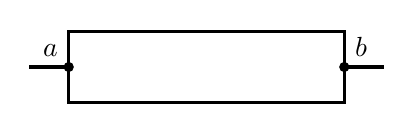
\begin{tikzpicture}[scale=.5, very thick]
        \draw (.5,.6) rectangle(7.5,2.4);
        \draw (-.5,1.5)--(.5,1.5);
        \draw (7.5,1.5)--(8.5,1.5);
        \fill(.5,1.5) circle(.13) node[above left] {$a$};
        \fill(7.5,1.5) circle(.13) node[above right]{$b$};
      \end{tikzpicture}\\
      Side View
      \vspace{.1in}
    \end{center}

    \part The electrons eventually experience no deflection and move through the
    bar at an average speed of \SI{3.5e-3}{\metre\per\second}.
    \textbf{Calculate} the strength of the additional electric field indicated
    in part \textbf{E}.
    \vspace{\stretch2}        
  \end{parts}
  \newpage

  % TAKEN FROM THE 2009 AP PHYSICS C EXAM FREE-RESPONSE QUESTION E&M 3
  % THIS IS A QUESTION ON MAGNETIC INDUCTION
  \uplevel{
    \centering
    \begin{tikzpicture}[scale=.8]
      \foreach\x in {0,...,3}{
        \foreach\y in {0,...,3} \node[gray] at (\x,\y){$\bm\times$};
      }
      \draw[thick](-.5,-.5) to[rmeter,t=1](-.5,3.5)--(3.5,3.5)
      to[rmeter,t=2] (3.5,-.5)--(-.5,-.5);
      \node at (1.5,1.5){$B$};
      \draw[thick,|<->|](-.5,3.85)--(3.5,3.85) node[midway,fill=white]{$L$};
    \end{tikzpicture}
  }
  
  \question A square conducting loop of side $L$ contains two identical
  lightbulbs, 1 and 2, as shown above. There is a magnetic field directed into
  the page in the region inside the loop with magnitude as a function of time
  $t$ given by $B(t)=at+b$, where $a$ and $b$ are positive constants. The
  lightbulbs each have constant resistance $R_0$. Express all answers in terms
  of the given quantities and fundamental constants.
  \begin{parts}
    \part\textbf{Derive} an expression for the magnitude of the emf generated
    in the loop.
    \vspace{\stretch1}
    
    \part\textbf{Determine} an expression for the current through bulb 2.
    \vspace{\stretch1}

    \part\textbf{Indicate} on the diagram above the direction of the current
    through bulb 2.
    \vspace{\stretch1}
    
    \part\textbf{Derive} an expression for the power dissipated in bulb 1.
    \vspace{\stretch1}
    
    \uplevel{
      Another identical bulb 3 is now connected in parallel with bulb 2, but it
      is entirely outside the magnetic field, as shown below.
      \begin{center}
        \begin{tikzpicture}[scale=.8]
          \foreach\x in {0,...,3}{
            \foreach\y in {0,...,3} \node[gray] at (\x,\y){$\bm\times$};
          }
          \draw[thick](-.5,-.5) to[rmeter,t=1](-.5,3.5)--(3.5,3.5)
          to[rmeter,t=2] (3.5,-.5)--(-.5,-.5);
          \draw[thick](3.5,3.5)--(5.5,3.5) to[rmeter,t=3](5.5,-.5)--(3.5,-.5);
          \node at (1.5,1.5){$B$};
          \draw[thick,|<->|](-.5,3.85)--(3.5,3.85) node[midway,fill=white]{$L$};
        \end{tikzpicture}
      \end{center}
    }

    \part How does the brightness of bulb 1 compare to what it was in the
    previous circuit?

    \vspace{.1in}
    \underline{\hspace{.3in}} Brighter\hspace{.5in}
    \underline{\hspace{.3in}} Dimmer\hspace{.5in}
    \underline{\hspace{.3in}} The same

    \vspace{.15in}\textbf{Justify} your answer.
    \vspace{\stretch1}
    \newpage
    
    \uplevel{
      Now the portion of the circuit containing bulb 3 is removed, and a wire is
      added to connect the midpoints of the top and bottom of the original
      loop, as shown below.
      \begin{center}
        \begin{tikzpicture}[scale=.8]
          \foreach\x in {0,...,3}{
            \foreach\y in {0,...,3} \node[gray] at (\x,\y){$\bm\times$};
          }
          \draw[thick](-.5,-.5) to[rmeter,t=1](-.5,3.5)--(3.5,3.5)
          to[rmeter,t=2] (3.5,-.5)--(-.5,-.5);
          \draw[thick](1.5,3.5)--(1.5,-.5);
          \node at (.5,1.5){$B$};
          \node at (2.5,1.5){$B$};
          \draw[thick,|<->|](-.5,3.85)--(3.5,3.85) node[midway,fill=white]{$L$};
        \end{tikzpicture}
      \end{center}
    }

    \part How does the brightness of bulb 1 compare to what it was in the first
    circuit?

    \vspace{.1in}
    \underline{\hspace{.3in}} Brighter\hspace{.5in}
    \underline{\hspace{.3in}} Dimmer\hspace{.5in}
    \underline{\hspace{.3in}} The same
  \end{parts}

  \vspace{.15in}\textbf{Justify} your answer.
  \newpage

  \uplevel{
    \centering
    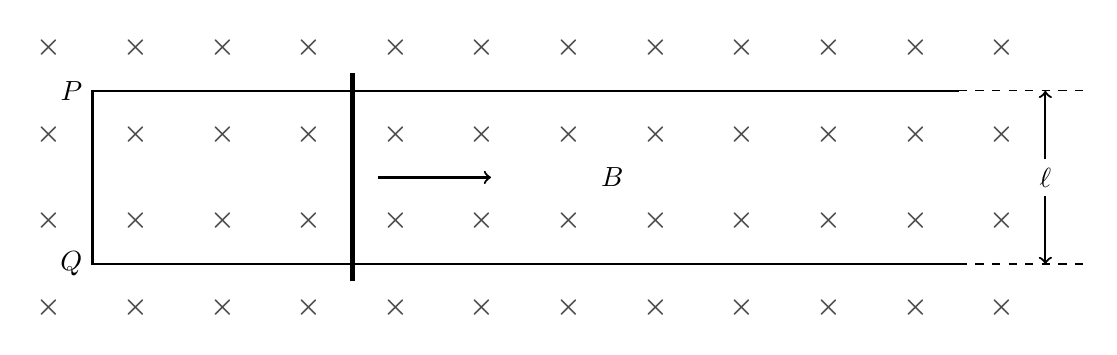
\begin{tikzpicture}[scale=1.1]
      \foreach \x in {0,...,11}
      \foreach \y in {0,...,3} \node[black!70] at (\x,\y) {$\bm\times$};
      \draw[thick](10.5,.5)--(.5,.5) node[left]{$Q$}--(.5,2.5) node[left]{$P$}
      --(10.5,2.5);
      \draw[dashed](10.5,2.5)--(12,2.5);
      \draw[dashed](10.5,0.5)--(12,0.5);
      \draw[ultra thick](3.5,.3)--(3.5,2.7);
      \node at (6.5,1.5) {$B$};
      \draw[thick,<->](11.5,.5)--(11.5,2.5) node[midway,fill=white]{$\ell$};
      \draw[thick,->](3.8,1.5)--(5.1,1.5) node[midway,above]{$\varv$};
    \end{tikzpicture}

    Top View
  }
  
  \question In the diagram above, a nichrome wire of resistance per unit length
  $\lambda$ is bent at points $P$ and $Q$ to form horizontal conducting rails
  that are a distance $\ell$ apart. The wire is placed within a uniform
  magnetic field of magnitude $B$ pointing into the page. A conducting rod of
  negligible resistance, which was aligned with end $PQ$ at time $t=0$, slides
  to the right with constant speed $\varv$ and negligible friction. Express all
  algebraic answers in terms of the given quantities and fundamental constants.
  \begin{parts}
    \part\textbf{Indicate} the direction of the current induced in the circuit.

    \vspace{.1in}
    \underline{\hspace{.3in}} Clockwise\hspace{.5in}
    \underline{\hspace{.3in}} Counterclockwise

    \vspace{.1in}\textbf{Justify} your answer.
    \vspace{\stretch1}
    
    \part\textbf{Derive} an expression for the magnitude of the induced current
    as a function of time $t$.
    \vspace{\stretch1}
    
    \part\textbf{Derive} an expression for the magnitude of the magnetic force
    on the rod as a function of time.
    \vspace{\stretch1}
    
    \part On the axes below, \textbf{sketch} a graph of the external force
    $F_\text{ext}$ as a function of time that must be applied to the rod to keep
    it moving at constant speed while in the field. \textbf{Label} the values
    of any intercepts.
    \begin{center}
      \begin{tikzpicture}
        \draw[axes] (0,0)--(7,0) node[right]{$t$} node[pos=0,below left]{$O$};
        \draw[axes] (0,0)--(0,4) node[above]{$F_\text{ext}$};
      \end{tikzpicture}
    \end{center}
    \newpage
    
    \part The force pulling the rod is now removed. \textbf{Indicate} whether
    the speed of the rod increases, decreases, or remains the same.

    \vspace{.1in}
    \underline{\hspace{.3in}} Increases\hspace{.5in}
    \underline{\hspace{.3in}} Decreases\hspace{.5in}
    \underline{\hspace{.3in}} Remains the same
    
    \vspace{.15in}\textbf{Justify} your answer.
  \end{parts}
\end{questions}
\end{document}
